%%
% The BIThesis Template for Bachelor Graduation Thesis
%
% 中国原子能科学研究院硕士学位开题报告模板 —— 使用 XeLaTeX 编译
%
% Copyright 2023 by Reni
%
% This work may be distributed and/or modified under the
% conditions of the LaTeX Project Public License, either version 1.3
% of this license or (at your option) any later version.
% The latest version of this license is in
%   http://www.latex-project.org/lppl.txt
% and version 1.3 or later is part of all distributions of LaTeX
% version 2005/12/0 1 or later.
%
% This work has the LPPL maintenance status `maintained'.
%
% The Current Maintainer of this work is Spencer Woo.
%
% This work consists of the files main.tex, misc/cover.tex and
% the external PDF misc/reviewTable.pdf
%
% Compile with: xelatex

\documentclass{article}
\usepackage[a4paper,left=3cm,right=2.4cm,top=2.6cm,bottom=2.38cm,includeheadfoot]{geometry}
\usepackage{fontspec}
\usepackage{setspace}
\usepackage{graphicx}
\usepackage{fancyhdr}
\usepackage{pdfpages}
\usepackage{setspace}
\usepackage{booktabs}
\usepackage{multirow}
\usepackage{caption}

\usepackage[utf8]{inputenc}
\usepackage[UTF8]{ctex}
\usepackage{subcaption}
\usepackage{url}

% 设置参考文献编译后端为 biber,引用格式为 GB/T7714-2015 格式
% 参考文献使用宏包见 https://github.com/hushidong/biblatex-gb7714-2015
\usepackage[style=gb7714-2015,backend=biber]{biblatex}

% 参考文献引用文件 refs.bib
\addbibresource{misc/refs.bib}

\newcommand{\deptName}{82801220001}
\newcommand{\majorName}{粒子物理与原子核物理}
\newcommand{\className}{2022级}
\newcommand{\yourName}{李费曼}
\newcommand{\mentorName}{波尔$\quad$麦克斯韦}

\newpage


% 文档开始
\begin{document}

% 报告封面
%%
% The BIThesis Template for Bachelor Graduation Thesis
%
% 中国原子能科学研究院硕士学位开题报告模板 —— 使用 XeLaTeX 编译
%
% Copyright 2023 by Reni
%
% This work may be distributed and/or modified under the
% conditions of the LaTeX Project Public License, either version 1.3
% of this license or (at your option) any later version.
% The latest version of this license is in
%   http://www.latex-project.org/lppl.txt
% and version 1.3 or later is part of all distributions of LaTeX
% version 2005/12/0 1 or later.
%
% This work has the LPPL maintenance status `maintained'.
%
% The Current Maintainer of this work is Spencer Woo.
%
% This work consists of the files main.tex, misc/cover.tex and
% the external PDF misc/reviewTable.pdf
%
% Compile with: xelatex

\topskip=0pt

\begin{titlepage}
  \vspace*{-16mm}
  \centering
  \hspace{-6mm}\songti\fontsize{22pt}{22pt}\selectfont\textbf{中国原子能科学研究院硕士学位研究生}

  \vspace{13mm}

  \hspace{-6mm}\heiti\fontsize{24pt}{24pt}\selectfont{开题报告}

  \vspace{33mm}
  
  \hspace{-6mm}\fontsize{18pt}{18pt}\selectfont{课题名称:中子辐射的影响及机制研究}

  \vspace{33mm}

  \flushleft
  \begin{spacing}{2.2}
    \hspace{25mm}\songti\fontsize{16pt}{16pt}\selectfont{\textbf{学\hspace{11mm}号:}\underline{\makebox[65mm][c]{\deptName}}}

    \hspace{25mm}\songti\fontsize{16pt}{16pt}\selectfont{\textbf{学科专业:}\underline{\makebox[65mm][c]{\majorName}}}

    \hspace{25mm}\songti\fontsize{16pt}{16pt}\selectfont{\textbf{年\hspace{11mm}级:}\underline{\makebox[65mm][c]{\className}}}

    \hspace{25mm}\songti\fontsize{16pt}{16pt}\selectfont{\textbf{姓\hspace{11mm}名:}\underline{\makebox[65mm][c]{\yourName}}}

    \hspace{25mm}\songti\fontsize{16pt}{16pt}\selectfont{\textbf{指导教师:}\underline{\makebox[65mm][c]{\mentorName}}}

    %\hspace{46mm}\songti\fontsize{16pt}{16pt}\selectfont{\textbf{校外指导教师:}\underline{\makebox[40mm][c]{\offCampusMentorName}}}
  \end{spacing}

  \vspace{40mm}

  \centering
  \hspace{-6mm}\songti\fontsize{18pt}{18pt}\selectfont{中国原子能科学研究院}
\end{titlepage}


% 评审表
%\includepdf[pages=-]{misc/reviewTableBlank.pdf}

%%
% 正文开始
\newpage
\begin{center}
    \tableofcontents
\end{center}% 目录

\newpage
\section{研究背景及意义}

\begin{figure}[!ht]
  \centering
  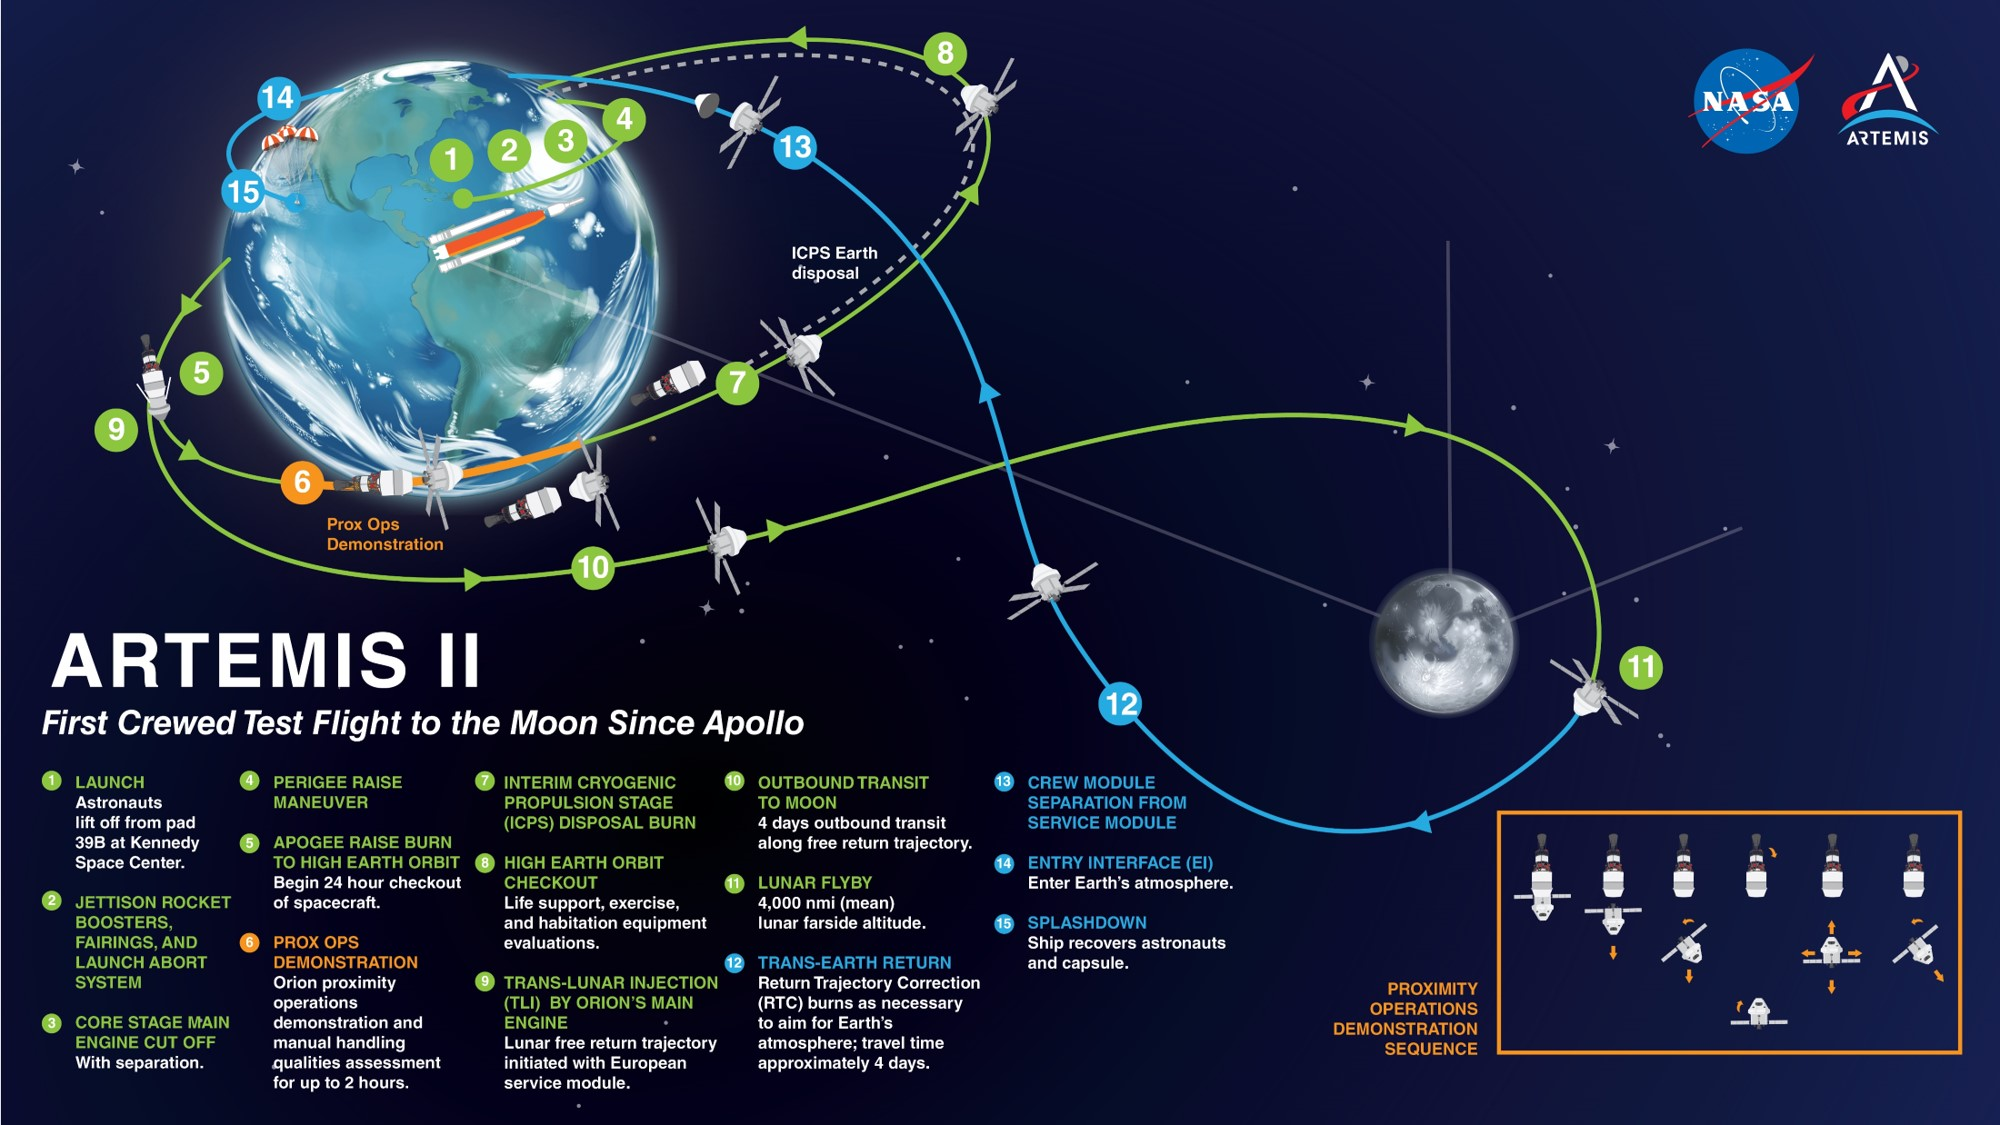
\includegraphics[width=0.6\linewidth]{artemis.jpg}
  \caption{Artemis}
  \label{fig:mergesort}
\end{figure}

\subsection{背景介绍}
下面先简要介绍下现有的方法。
\cite{2019space}。

\newpage
\section{国内外研究现状}



\newpage
\section{研究目标及研究方案}
\subsection{研究方案}

\subsection{研究方案}

\newpage
\section{技术路径及研究基础}
\subsection{技术路径}

\subsection{研究基础}
\subsubsection{实施技术方案所需的条件}
说明所需的软硬件等设施。

\begin{table}[!ht]
  \centering
  \caption{环境设施}
  \label{tab:soft-hardware}
  \begin{tabular}{@{}lcl@{}}
    \toprule
    & 指标     & \multicolumn{1}{c}{版本参数} 
    \\ \midrule
    \multirow{2}{*}{环境} & 硬件 & \begin{tabular}[c]{@{}l@{}}CPU Intel i7-6500U
    \\  RAM 8 GB\end{tabular} 
    \\ \cmidrule(l){2-3}  & 软件 & Python 3.7.6  
    \\ \midrule
    \multirow{1}{*}{设施} & 物理装置 & \begin{tabular}[c]{@{}l@{}}HI-13串流加速器
    \\  回旋加速器\end{tabular}    
    \\ \bottomrule
  \end{tabular}
\end{table}

\newpage
\section{创新点与预期成果}
\subsection{创新点}

\subsection{预期成果}

\newpage
\section{研究进度}
\subsection{课题计划进度表}
大致的课题计划进度如下表 \ref{tab:progress} 所示。

\begin{table}[!ht]
  \centering
  \caption{毕业设计计划进度表}
  \label{tab:progress}
  \begin{tabular}{@{}cllc@{}}
    \toprule
    阶段 & \multicolumn{1}{c}{任务} & \multicolumn{1}{c}{完成标志} & 时间规划       \\ \midrule
    1    & 第一阶段的任务……          & 成功搭建……                    & 2019.12-2020.1 \\ \midrule
    2    & 第二阶段的任务……          & 成功验证……                    & 2020.1-2020.2  \\ \midrule
    3    & 第三阶段的任务……          & 成功验证……失效,并优化……增强  & 2020.2-2020.4  \\ \midrule
    4    & 第四阶段的任务……          & 成功完成毕业设计              & 2020.4-2020.5  \\ \bottomrule
  \end{tabular}
\end{table}


\newpage
\setcounter{secnumdepth}{0}  %开始一段不带编号的章
\begin{center}
    \section{参考文献}
\end{center}


\printbibliography[heading=none]




\end{document}